% Auto-generated by make_figures.py -- residual phi per defense
\pgfplotsset{width=\linewidth,height=6cm,compat=1.16}
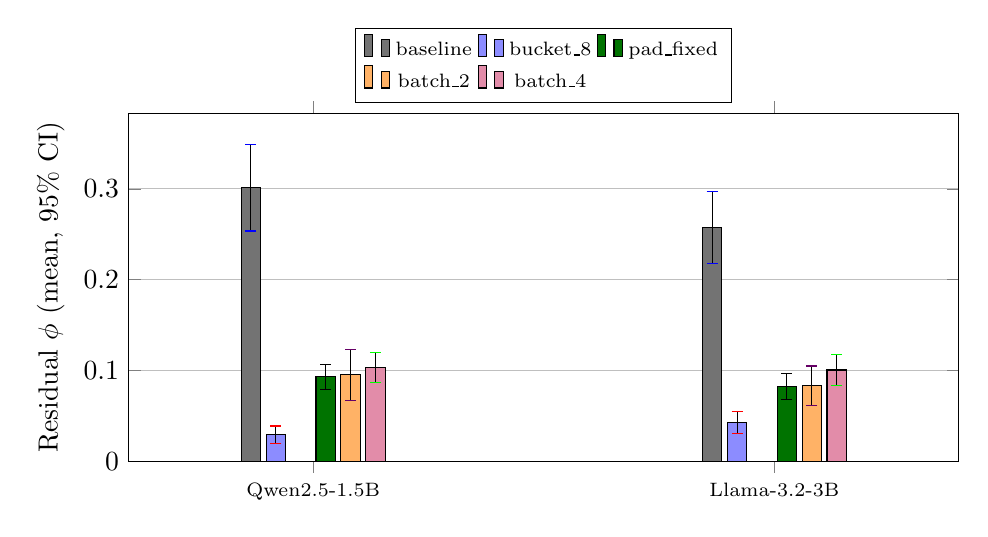
\begin{tikzpicture}
\begin{axis}[
  ybar, bar width=7pt, ymin=0,
  ylabel={Residual $\phi$ (mean, 95\% CI)},
  symbolic x coords={Qwen2.5-1.5B,Llama-3.2-3B},
  xtick=data, x tick label style={font=\scriptsize},
  legend style={font=\scriptsize,at={(0.5,1.03)},anchor=south,legend columns=3},
  ymajorgrids, enlarge x limits=0.4,
]
\addplot+[ybar,fill=black!55,draw=black,
  error bars/.cd, y dir=both, y explicit] coordinates {(Qwen2.5-1.5B,0.3010) +- (0.0498,0.0474) (Llama-3.2-3B,0.2576) +- (0.0402,0.0399)};
\addlegendentry{baseline}
\addplot+[ybar,fill=blue!45,draw=black,
  error bars/.cd, y dir=both, y explicit] coordinates {(Qwen2.5-1.5B,0.0293) +- (0.0104,0.0095) (Llama-3.2-3B,0.0428) +- (0.0135,0.0123)};
\addlegendentry{bucket\_8}
\addplot+[ybar,fill=red!45,draw=black,
  error bars/.cd, y dir=both, y explicit] coordinates {};
\addlegendentry{pad\_fixed}
\addplot+[ybar,fill=green!45!black,draw=black,
  error bars/.cd, y dir=both, y explicit] coordinates {(Qwen2.5-1.5B,0.0928) +- (0.0144,0.0137) (Llama-3.2-3B,0.0823) +- (0.0144,0.0139)};
\addlegendentry{batch\_2}
\addplot+[ybar,fill=orange!60,draw=black,
  error bars/.cd, y dir=both, y explicit] coordinates {(Qwen2.5-1.5B,0.0950) +- (0.0318,0.0283) (Llama-3.2-3B,0.0832) +- (0.0224,0.0217)};
\addlegendentry{batch\_4}
\addplot+[ybar,fill=purple!45,draw=black,
  error bars/.cd, y dir=both, y explicit] coordinates {(Qwen2.5-1.5B,0.1033) +- (0.0170,0.0162) (Llama-3.2-3B,0.1004) +- (0.0182,0.0170)};
\addlegendentry{rand\_pad\_8}
\end{axis}
\end{tikzpicture}
